\documentclass[12pt]{article}
\textheight=8.5in
\textwidth=6.5in
\topskip=-0.55in
%\voffset=-0.75in
\def\h{\frac12}

\usepackage{graphicx}
\usepackage{amsmath}
\usepackage{amssymb}
\usepackage{amsthm}
\usepackage[dvips]{epsfig}
\usepackage{geometry}
\usepackage{color}

\newcommand{\Fig}[1]{Figure~\ref{#1}}

\begin{document}

\centerline{\Large\bf How to make a movie using VisIt}
\vskip 1.5cm

This manual shows how to use VisIt to make an animated movie from 
{\it FronTier++} generated vtk files. In each run, {\it FronTier++} 
generated vtk files are stored in the
out-{\it RunName}/vtk directory. To make movie using VisIt, follow 
the steps described below.

\begin{itemize}
\item[(1).] Interface Plot.
"2d-intfc.vtk" is for 2D movie, "3d-intfc.vtk" is for 3D movie and 
they are all in the vtk folder after a {\it FronTier++} run.

You also need a list file for these files, for example, "vtk.visit".
The file "vtk.visit" includes every "2d-intfc.vtk" or "3d-intfc.vtk" 
in each output time step. For example, you may have: 

\noindent
vtk.ts0000030/3d-intfc.vtk \\
vtk.ts0000060/3d-intfc.vtk \\
vtk.ts0000090/3d-intfc.vtk \\

To make "vtk.visit", you can use the script file that can be found in this
directory "visit.bash". After generating the "vtk.visit" from the
script file, start VisIt. Then open "vtk.visit", using the command
File$\rightarrow$Open File and choose vtk.visit. See \Fig{fig:image1}.

After this click, the file "vtk.visit" is activated.
You should then click the 'Plots' button and choose what you would like to
plot. For example, we can choose 'mesh$\rightarrow$mesh' and click 'Draw'.
You can choose 'Pseudocolor', 'Surface' etc. See \Fig{fig:image2} and 
\Fig{fig:image3}.

You can the see the interface in the window such as in \Fig{fig:image4}.
You can change the scale or view angle using mouse.

At this point, click the play button, the animated images will be
shown frame by frame. See \Fig{fig:image5}.

To save the movie, click 'file$\rightarrow$Save movie', see 
\Fig{fig:image6}.

Choose 'New simple movie' and choose output format and add to output
window. Click 'next' button to move on (\Fig{image7}).

Choose 'Now, use a new instant VisIt’ to finish saving the movie file.
See \Fig{fig:image8}.

If you quit VisIt now, you will have all the jpeg files in
your local directory. You can use ‘convert’ command to make a ‘.gif’ file.

convert *.jpeg MovieName.gif

This complete your movie production procedures.

\item[(2).] Vector plot. Vector vtk files are used to make movie 
showing the evolution of a vector field such as the velocity or force
field. {\it FronTier++} will generate the Velo.vtk files in the vtk
directories and can be used for this type of movies.
The movie production procedures are similar to interface plot, 
but this time, it uses velocity files. For example, you need to have
the velo.visit file containing

\noindent
vtk.ts0000030/velo.vtk \\
vtk.ts0000060/velo.vtk \\
vtk.ts0000090/velo.vtk \\

Run VisIt and open your velo.visit file in the same way as 
you do for the interface plot, but you need to choose different 
plot type: ‘Plots$\rightarrow$Vector$\rightarrow$Velocity’, see
\Fig{fig:image9}.

Click DRAW, then you can see the vector field plot on the window.
When you click play button, you will see the animation. To save the
movie, use the same procedures as in (1).

\item[(3).] Movie from a parallel run. For making a movie from 
parallel run, we just need one more line on the top of ‘vtk.visit’ 
or ‘velo.visit’ file with

\noindent
!NBLOCKS=node number

For example, if you have used 64 processors for a parallel run, 
you should to make a vtk.visit file as follows;

\noindent
!NBLOCKS=64 \\
vtk.ts0000001-nd0000/3d-intfc.vtk \\
vtk.ts0000001-nd0001/3d-intfc.vtk \\
vtk.ts0000001-nd0002/3d-intfc.vtk \\
vtk.ts0000001-nd0003/3d-intfc.vtk \\
vtk.ts0000001-nd0004/3d-intfc.vtk \\

Then the rest of the procedures are the same as in (1) and (2).



\begin{figure}[!h]
\centering
\begin{tabular}{l}
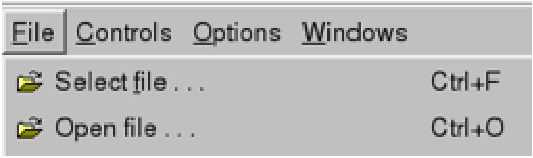
\epsfig{file=image1,width=0.4\hsize}
\end{tabular}
\caption{Open file menu.}
\label{fig:image1}
\end{figure}

\begin{figure}[!h]
\centering
\begin{tabular}{l}
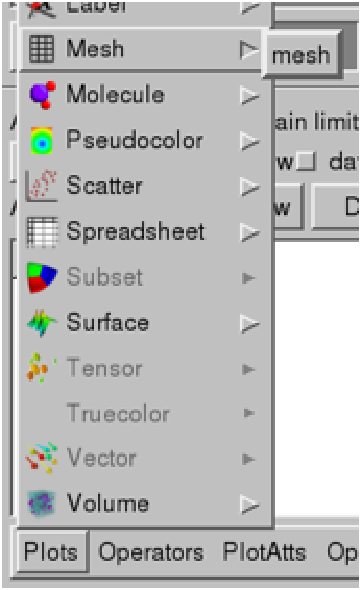
\epsfig{file=image2,width=0.4\hsize}
\end{tabular}
\caption{Choose plot type.}
\label{fig:image2}
\end{figure}

\begin{figure}[!h]
\centering
\begin{tabular}{l}
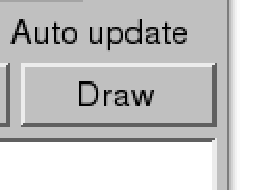
\epsfig{file=image3,width=0.4\hsize}
\end{tabular}
\caption{Draw.}
\label{fig:image3}
\end{figure}

\begin{figure}[!h]
\centering
\begin{tabular}{l}
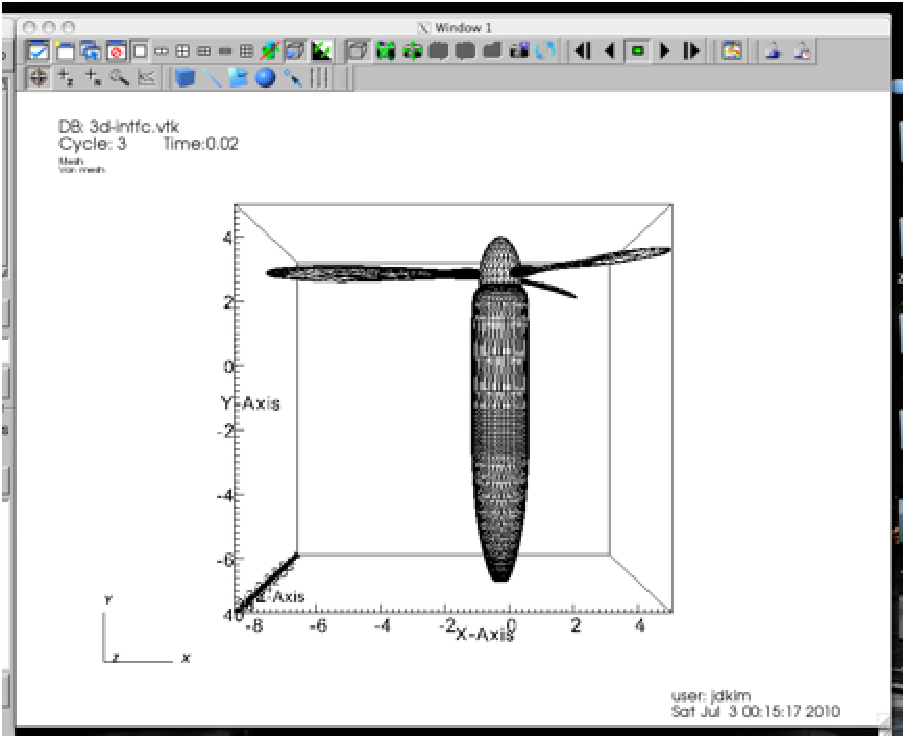
\epsfig{file=image4,width=0.4\hsize}
\end{tabular}
\caption{First image, can scale and rotate.}
\label{fig:image4}
\end{figure}

\begin{figure}[!h]
\centering
\begin{tabular}{l}
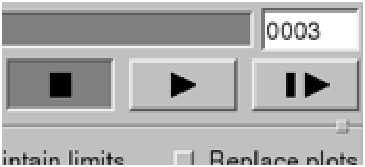
\epsfig{file=image5,width=0.4\hsize}
\end{tabular}
\caption{The play button is the middle one.}
\label{fig:image5}
\end{figure}

\begin{figure}[!h]
\centering
\begin{tabular}{l}
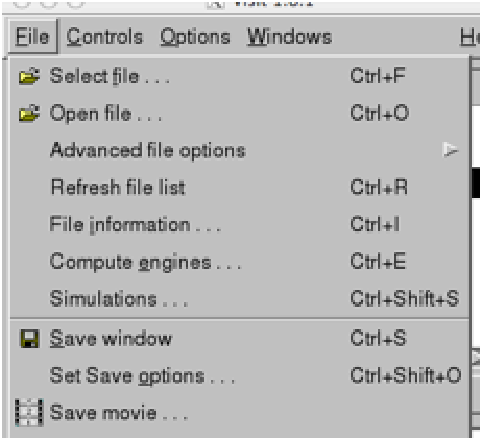
\epsfig{file=image6,width=0.4\hsize}
\end{tabular}
\caption{Save movie.}
\label{fig:image6}
\end{figure}

\begin{figure}[!h]
\centering
\begin{tabular}{l}
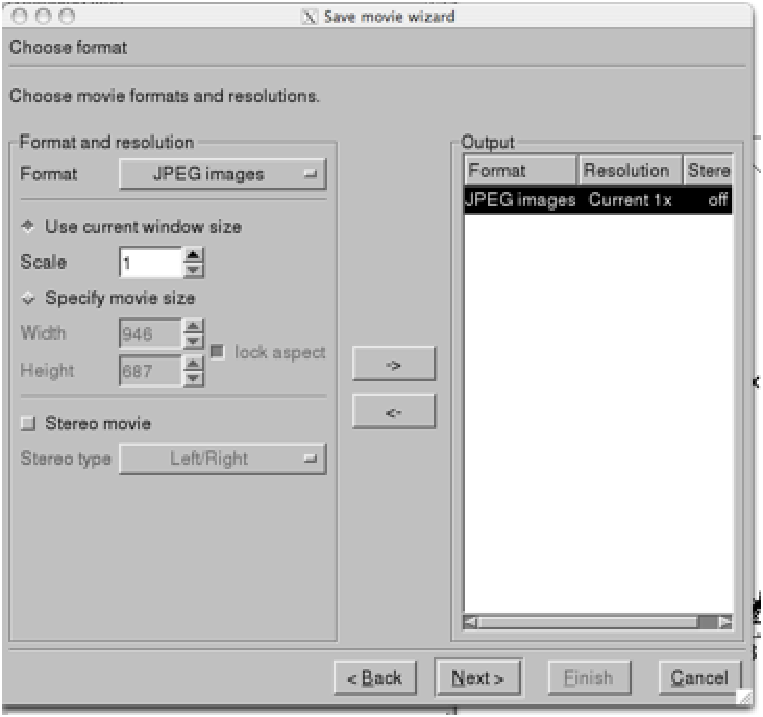
\epsfig{file=image7,width=0.4\hsize}
\end{tabular}
\caption{File type.}
\label{fig:image7}
\end{figure}

\begin{figure}[!h]
\centering
\begin{tabular}{l}
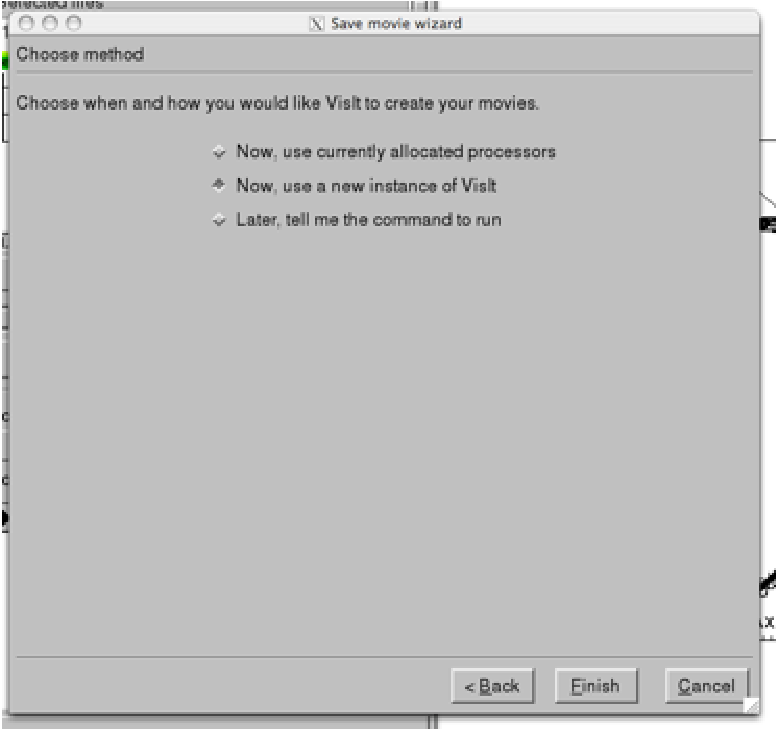
\epsfig{file=image8,width=0.4\hsize}
\end{tabular}
\caption{Finish visit.}
\label{fig:image8}
\end{figure}

\begin{figure}[!h]
\centering
\begin{tabular}{l}
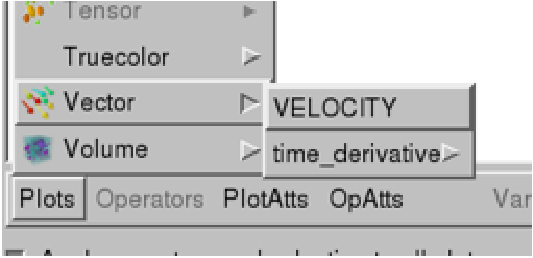
\epsfig{file=image9,width=0.4\hsize}
\end{tabular}
\caption{Choose vector plot}
\label{fig:image9}
\end{figure}



\end{itemize}
\end{document}
